\chapter{Theory}

\section{Moon Characteristics} % JP, Yannis

% General info: https://en.wikipedia.org/wiki/Colonization_of_Europa

\iffalse
* Rock core, water, ice

    * Why do we think so?
    
    * Geysers?
\fi 

\subsection{Radiation Environment} \label{chap:radiation}%  "landing site guys", "orbiter guys"

%* Both for the orbiter and the lander

Radiation: http://zimmer.csufresno.edu/~fringwal/w08a.jup.txt

\autsubsection{Tidal Wave}{Kristian Sloth Lauszus and Lukas Christensen}

\section{Ice characteristics}

\subsection{Structural Profile}
The first space probe flybys took place in the early 1970s, and Europa quickly became one of the main focuses in the search for past or present extraterrestrial life-harbouring environments, within reachable distances. Already in the 1960's were it discovered from earth-based observations, that the surface of Europa was covered in solid ice, not much unlike other satellites located that deep in the cold reaches of our solar-system. However, data recovered from satellite flybys supplied us with new information about the geology and composition of the moon's surface, having since helped us understanding the of Jupiter's, arguably, most interesting moons with respect to life-supporting environments.\\
\\
The Voayger mission from the late 1970's sent back coarse imagery of Europa with resolution in the ranges of kilometres per pixel, carrying valuable information about the surface of the Jovian satellite\cite{VoyagImg}. More specifically, the images showed a surface resembling that of a ball of string, discarding theories of Europa having a smooth surface, with it in stead being full of bands and ridges.\\%See requested article from DTU Findit
The Galileo spacecraft was launched in 1989 and entered orbit around Jupiter in 1995. It started transmitting data back to earth, from its extensive remote-sensing instrument suite
\iffalse 
(seen on fig. \ref{fig:GalInst1} and \ref{fig:GalInst2})
\fi
 with resolution surpassing Voayger's images almost three orders of magnitude. 
\iffalse
\begin{figure}[htb]
	\centering
	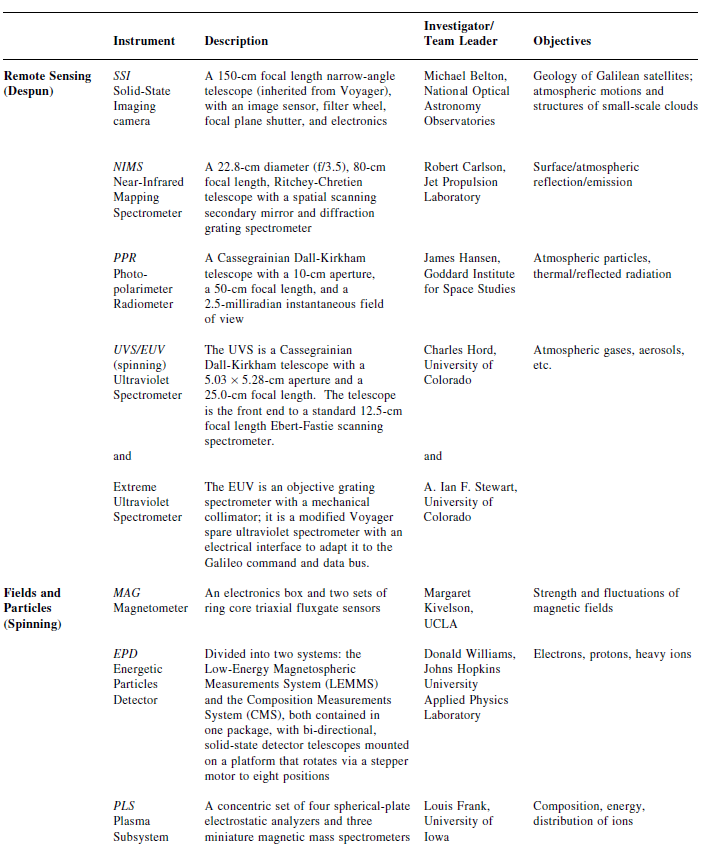
\includegraphics[width=\textwidth]{figures/Rasmus/GalileoInstrument1}
	\caption{Instrument suite of the 1989 Galileo mission.\cite{SciStrat} (\textit{Continued in fig. \ref{fig:GalInst2}}). \label{fig:GalInst1}}
\end{figure}
\begin{figure}[htb]
	\centering
	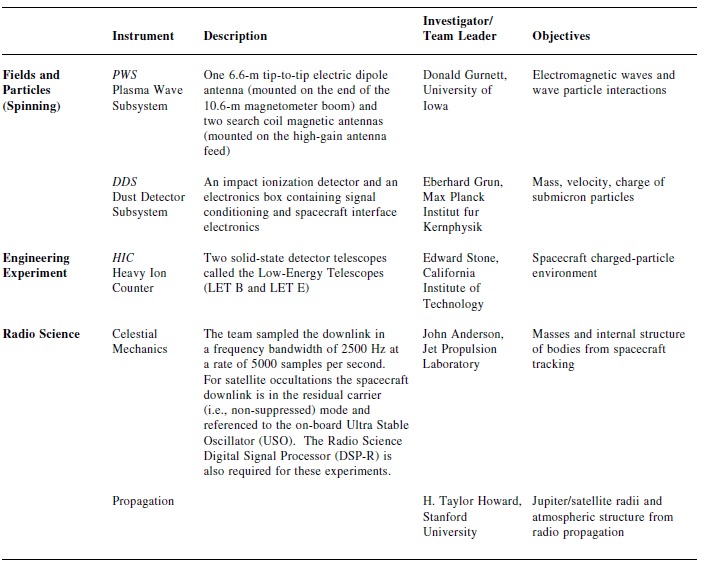
\includegraphics[width=\textwidth]{figures/Rasmus/GalileoInstrument2}
	\caption{Instrument suite of the 1989 Galileo mission.(Continued from fig. \ref{fig:GalInst1}) \cite{SciStrat} .\label{fig:GalInst2}}
\end{figure}
\fi
\\
The high-resolution measurements showed what seemed to be blocks of ice filled with ridges and/or early cracks, that had been lifted and rotated at some point in time. These disruptions indicates that there might be a liquid or softer slushy layer underneath the solid ice surface that through movement had broken and relocated the ice-crust. These cracks are illustrated on fig. \ref{fig:SurfCrack}, which is one picture of a series from the 1989 Galileo satellite\cite{HidOcean}. In any case, it indicates that there is some kind of structural activity in the outermost layer of the moon.\\
\\

\begin{figure}[htb]
	\centering
	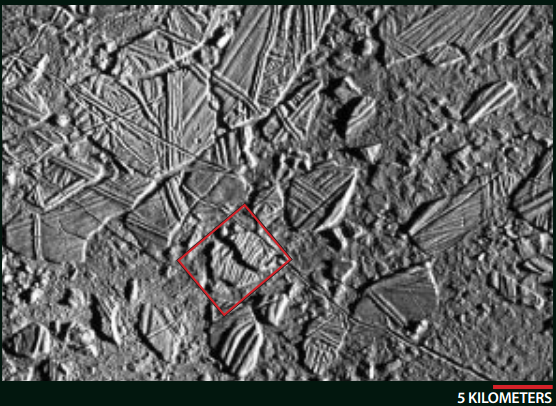
\includegraphics[width=\textwidth]{figures/Rasmus/SurfCrack}
	\caption{Image of Europa's surface taken by the Galileo satellite, showing ridges and disruptions in the surface. \label{fig:SurfCrack}\cite{HidOcean}}
\end{figure}

% Surface Composition
As explained in the study made by the Space Studies Board's Committee on Planetary and Lunar Exploration (COMPLEX), the data from Galileo’s Near-Infrared Mapping Spectrometer (NIMS) show that the water-ice absorption of Europa doesn't match with the expected outcome of pure-water ice, even for areas where the level of frozen sulfur oxide is thought to be lowest (The source of this $SO_2$ is presumably volcanic eruption on Io.). There has been some theories on the cause of this, including the presence of salts and other minerals in the ice but recent studies show that bubbles and fractions could result in the same discrepancies and band shifts in the measurements. However, it is still believed that some of the darker spots seen on the moon are observed because of salts and minerals like hexahedrite, epsomite, and natron\cite{SciStrat}. % INDSÆT The identity of that contaminant so far eludes scientists, but sulfur or iron compounds are suspected from Hidden Ocean P. 8
\\
\\
The actual thickness of the theorized ice-crust, and even the complete structural model of the moon, is still subject to many discussions. It was previously (prior to the Galileo mission) believed that the moon could be consisting of a hydrated silicate core coated in a thin layer of water-ice. However, with the measurements of Europa's gravitational field done by the Galileo satellite has this theory since been largely debunked. The current popular belief is that the cores is either a solid or fluid metallic core surrounded by a layer of water and ice of more than 100km due to the estimated density of the Jovian body. \\
The global ratio between liquid and solid water-ice is still unknown since it must be based on assumptions about the internal structure of the ice, which in themselves are extremely uncertain. The estimates we do have are even based on local imagery, since making them on a global basis requires dedicated orbiter mission, like the planned CLIPPER mission.\\%INDSÆT REFERENCE
In one study, the impact craters of Europa are analysed and compared with computer simulations to estimate regional crust thickness. The rationale is, that central peaks found in craters on the surface resemble material uplift caused by meteor impacts on extraterrestrial planets\cite{ThickImpact}, as seen on fig. \ref{fig:ImpactPic}. Therefore, it is assumed that the crust is thick enough to prevent complete surface penetration from meteor impact and as such they conclude that the ice at the impact sites must have been more than 	$\mathbf{3-4km}$ thick. Graphical representation of the simulation results can be seen on fig. \ref{fig:ImpactSim}. Another study that also investigated the impact craters, and taken from their introduction: "Stereo topographic profiles suggest that the plateau [a plateau SW of Cilix impact crater] is
flexurally supported, with an effective elastic thickness $t_e$ of
$~6km$. For a conductive temperature profile this $t_e$ value
implies a solid ice shell thickness of $\mathbf{~15km}$; if the shell is
convecting, this estimate is a lower bound. Combined with
independent estimates, we infer a probable shell thickness
of $\mathbf{25 km}$. The shell thickness is likely to be uniform over
the entire satellite."\cite{ThermElast}
\begin{figure}[htb]
	\centering
	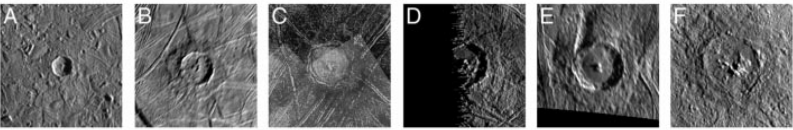
\includegraphics[width=\textwidth]{figures/Rasmus/Impacts}
	\caption{Galileo images of Europan central peak craters. (\textbf{A}) Brigid ($11^\circ$N, $80^\circ$W), $D=8.5km$. (\textbf{B}) Grainne ($60^\circ$S, $95^\circ$W), $D=13.5$km. (\textbf{C}) Cilix ($2.6^\circ$N, $182^\circ$W ), $D18.4$km. (\textbf{D}) Amergin ($14^\circ$S, $230^\circ$W), $D=18.6$km. (\textbf{E}) Maeve ($58^\circ$N, $75^\circ$W ), $D=20.4$km. (\textbf{F}) Pwyll ($25^\circ$S, $271^\circ$W), $D=23.7$ km. All images are at a resolution of 250 m/pixel and each is illuminated from the right except Cilix (\textbf{C}), which was observed at high sun
	\cite{ThickImpact}. D is crater diameter. \label{fig:ImpactPic}}
\end{figure}
\begin{figure}[htb]
	\centering
	\includegraphics[width=1\textwidth]{figures/Rasmus/Impacts2}
	\caption{Model results for impacts of large (A through C) and small projectiles (D through F) into 9-km-thick ice (gray) over liquid water (A) and (D), 5-kmthick ice (gray) over liquid water (black) (B) and (E), and 3-kmthick conductive lid (light gray) over convecting ice (dark gray) (C) and (F). Solid, dotted, and dashed lines show the regions of complete vaporization, complete melting, and $50\%$ melting, respectively.
	\cite{ThickImpact}.\label{fig:ImpactSim}}
\end{figure}
\\
Thermal models has also been used to estimate the average ice shell thickness of Europa. One study is carried out with the assumption of a ice shell decoupled from a silicate core by a layer of liquid water \cite{ThermThick}, so its conclusion may not fit with modern theories. They estimate the shell to have a thickness of $\mathbf{13-25km}$, depending on which thermal rheology model is used (Maxwell and general flow rheology, with and without heat flow from the core). Another thermal model is based on the suggestios of Europa having a metallic core and a silicate mantle, covered by significant layer of liquid water and a thinner ice shell \cite{ThermThick2}. The study heavily relies on convection in the ice, and this complicates the study further. The heat flow through the ice is dependant on the shell thickness, and shell thickness is in turn dependant on the heat flow. This study concludes on the result that the average thickness of a completely frozen shell must be around $\mathbf{36km}$ based on the study's assumptions.
\\
\\ One study carried out by [J.M. Wahr, M.T. Zuber et al., 2006] analyses the tidal effects caused by the differentiating gravitational pull from Jupiter, as Europa travels in its elliptical orbit around the planet. The result of the study is a set of analytical equations estimating the global thickness based on the Love-number of Europa. However, in order to utilize these equations, accurate knowledge of the ice-composition is required, as well as precise estimates of the Love numbers. In the end they even conclude conclude that their results may not be sufficient since they only provide an accuracy of $\pm 5\mathrm{km}$.\\
\\
Apart from the thickness and elemental composition of the ice, internal structure in the shelf is also highly relevant to the planned penetrator mission. Assuming a completely homogeneous ice-shelf is a crude over-simplification and may be a mission-killer if alternatives aren't considered. 
\begin{figure}[htb]
	\centering
	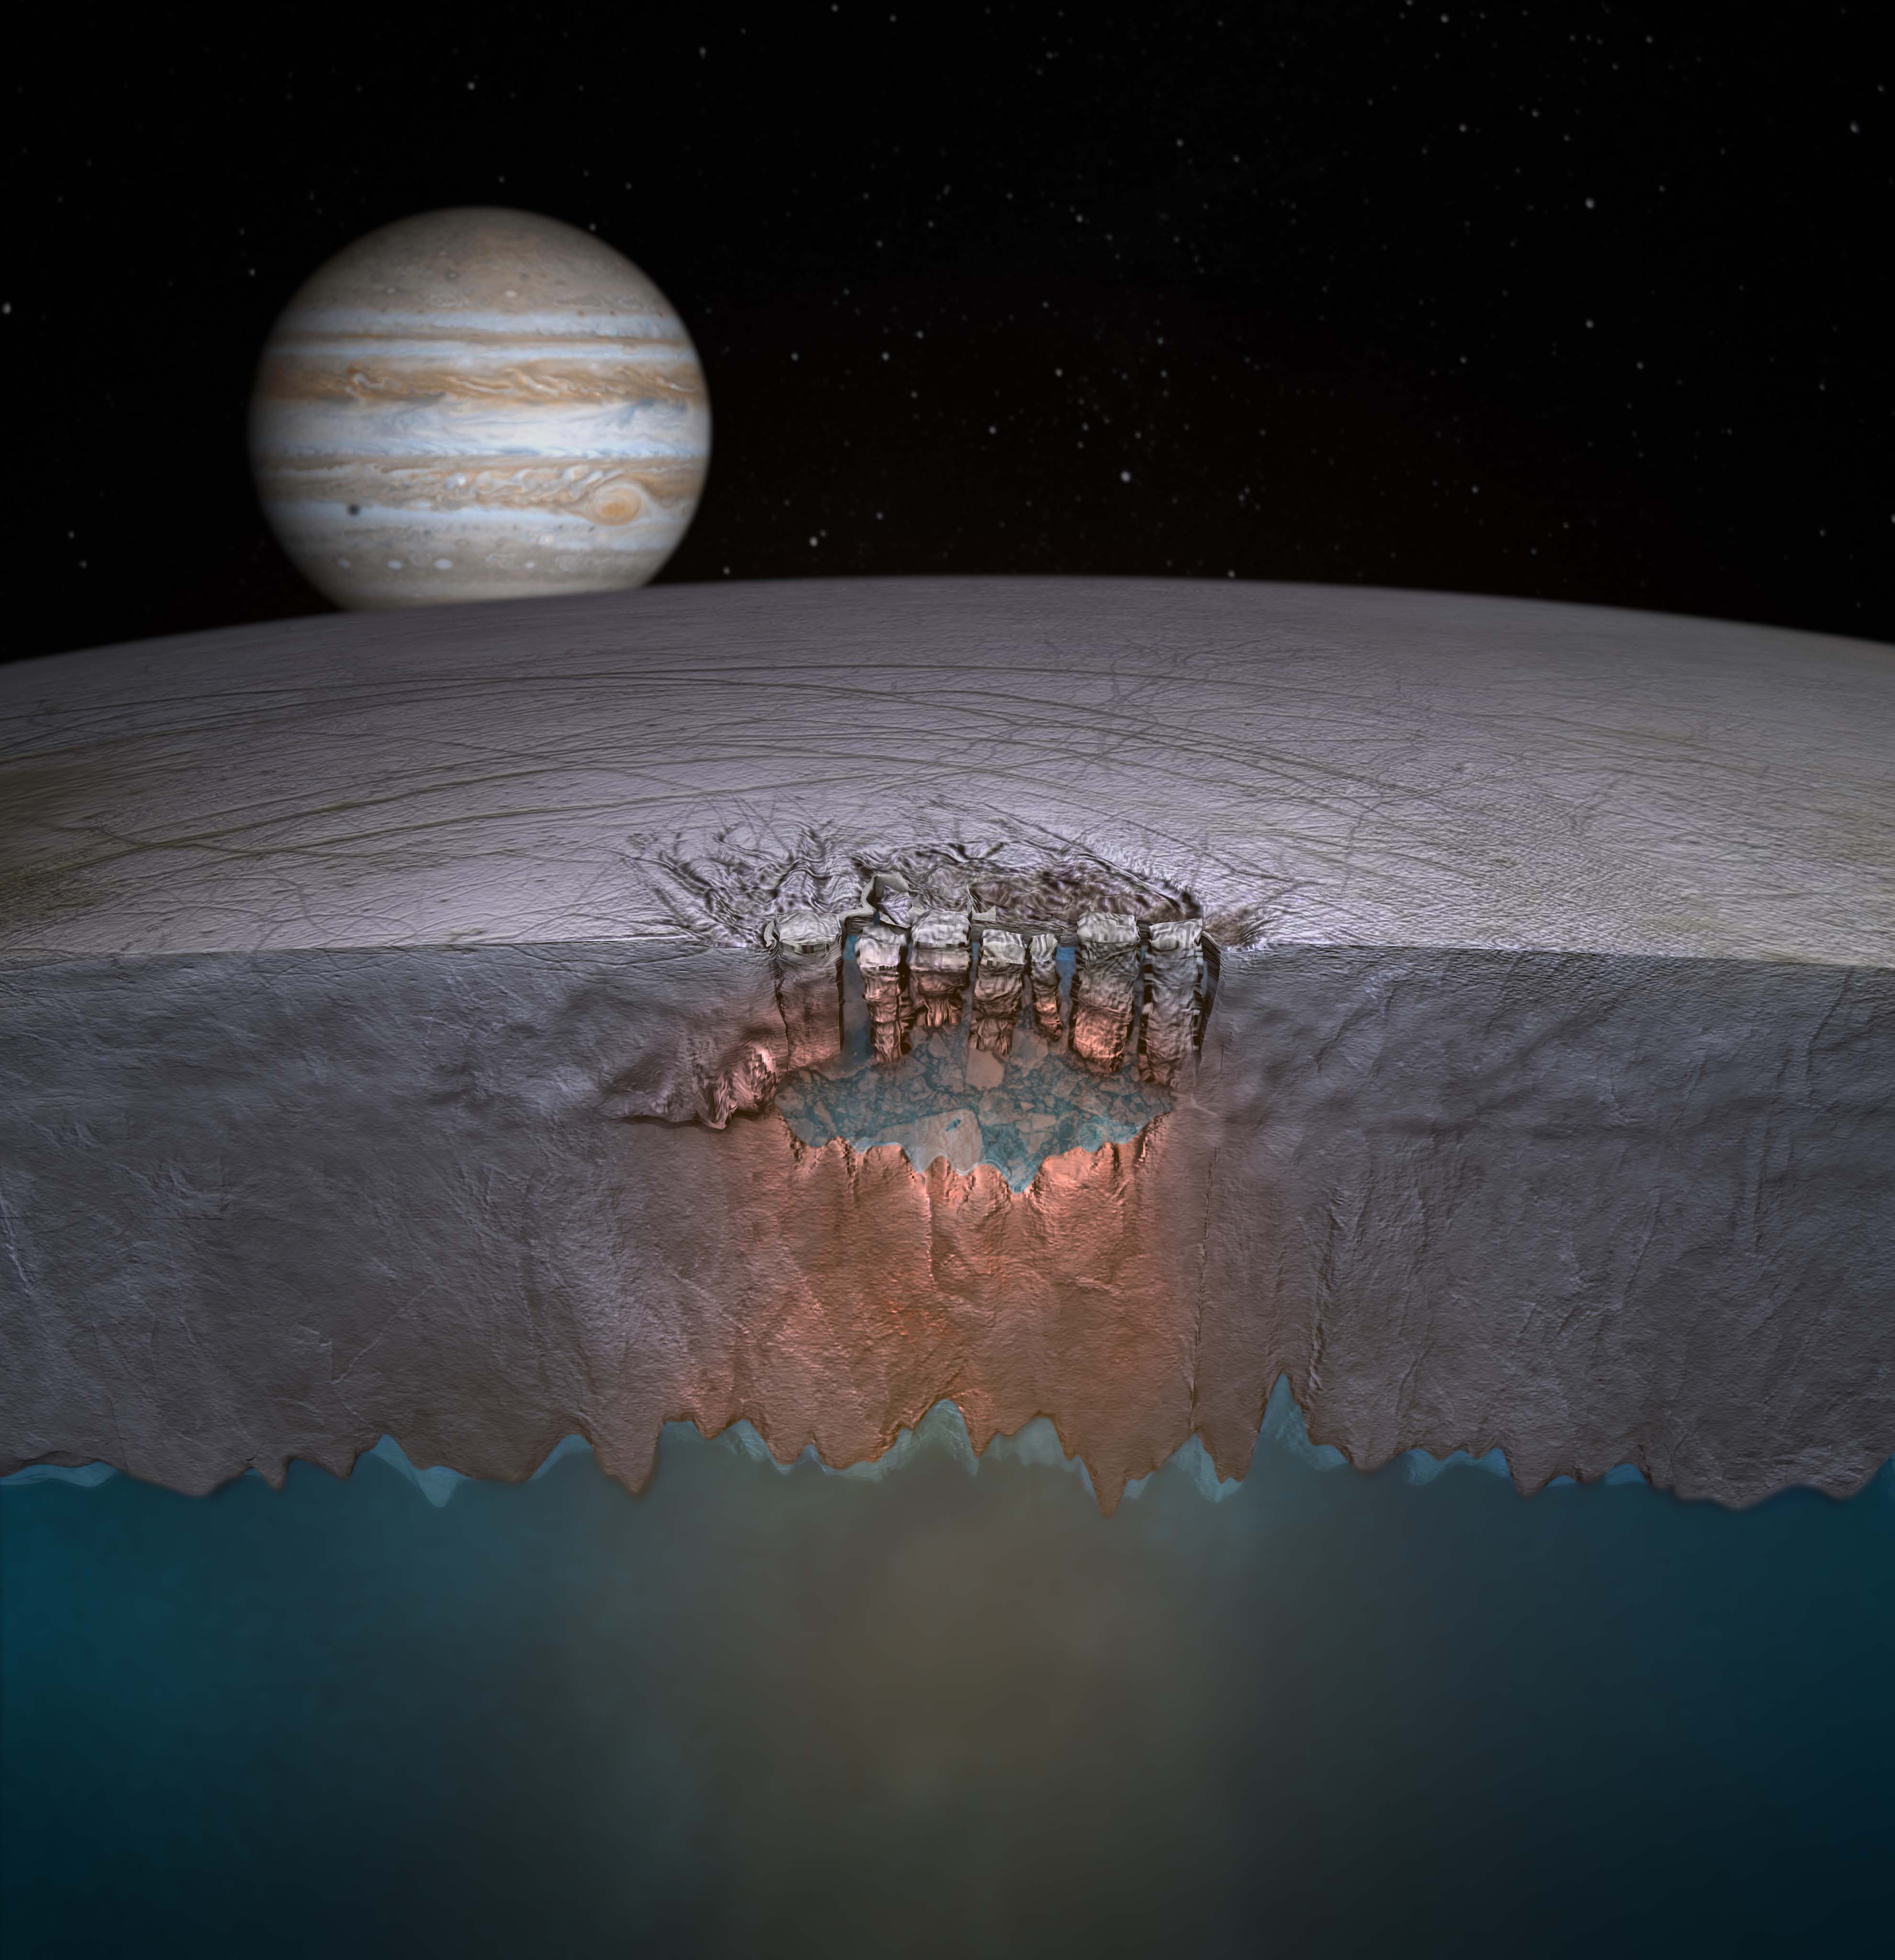
\includegraphics[width=0.5\textwidth]{figures/Rasmus/ArtLake}
	\caption{Artistic illustration of potential water lense, or lake, in the ice shell. \label{fig: ArtLake}}
\end{figure}
As such, apparent "Chaos Regions" has been observed on the surface of Europa and their causes has for a long time alluded scientists. However, recent studies suggests that these are formed due to water lenses in the shell, which can also be interpreted as lakes of liquid water \cite{IceLakes}. They way even be present within $3km$ of the surface, and it is estimated that there may be a water lense consisting of $20,000 - 60,000km^3$ of liquid water beneath the so-called Thera Macula chaos region. An artistic illustration of this phenomenon is shown on fig \ref{fig: ArtLake}.

\iffalse
* Ice thickness

* Composition of the ice? % Se: SWRI: "barr-showman-2009" (ask Kristian Lauszus)

* Lakes?
\fi

\subsection{Temperature Profile}

* "back of the envelope" calculations

\subsection{Pressure Profile}

* What is the outside pressure?

\subsection{Simulation Results}

\subsection{Simulation Validation}

* Should show that the "back of the envelope" calculations are right

\chapter{Defining Life}

One of the main objectives, if not the main objective, on this mission is to search for life. This is after all a life finding mission and therefore the instrument suite onboard needs to be focused on finding life. The mission is going to look for life in the ice and mostly in the water below the ice, where there is a high expectancy to find some sort of life or life harbouring conditions. \par
Life can be found in many forms and stages of evolution, and it can therefore be very difficult to detect, because we do not know exactly what the penetrator should look for. Before looking into what we should look for on Europa, a set of guide rules needs to be put in place, defining what life forms are already known from earth. It would be ideal to set up a precise yardstick for life, a list of things needed to say that life will exist, but this is not possible. What is possible is to look at what is present on Earth and applying this to alien life forms. \par
Most living organisms as we know from Earth have some properties in common, though non-living matter show some of them, only living organisms show all of them\footnote{$https://da.khanacademy.org/science/biology/intro-to-biology/what-is-biology/a/what-is-life$ 22-05-2016}. The 7 properties are: \par

\begin{enumerate}
  \item Organization
  \item Metabolism
  \item Homeostasis
  \item Growth
  \item Reproduction
  \item Response
  \item Evolution
\end{enumerate}

Beginning at number one “Organization”, to have life, structure is needed, and by taking unorganized matter and organizing it, is a sign of life. Living organisms a made up of one or more cells which in them self are highly organized, and able to produce complex chemical processes from an unorganized energy source. For bigger multi-cell organisms, organization is important, since individual cells are assigned different specific jobs to create a bigger and more complex organism. \par  
Metabolism is the life sustaining chemical transformations happening within cells and living organisms, and is the sum of all chemical reactions happening in a living organism. This chemical conversion can be divided into two subcategories, catabolism and anabolism. Catabolism is the process of breaking down organic matter into energy, with anabolism being the reverse process, building up complex molecules such as protein from simple molecules. This type of process uses energy. One of the most important metabolisms, is the citric acid cycle (Krebs cycle), it is believed to be one of the early established components for cellular metabolism. \par
Most living cells and organisms have a working area where they are able to sustain life; humans need to stay a cool 37 degrees to function normally. The ability to maintain a stable internal environment, even with a varying external environment is called homeostasis. This type of process is mostly found in more complex organisms, like smaller animals. Microorganisms usually depend on their surroundings to create a stable living environment.\par
The fourth properties is growth, this begins at a cellular level and is linked to the organization of the cells in defined structures. It depends on the anabolism to crate proteins and amino acids for DNA. Without growth more complex molecules and organisms would not exist.\par
Reproduction is also important for sustained life, looking at single cell organism like bacteria, which is able to reproduce by simply splitting in two. Reproduction can also take place with two parent organisms creating a new cell from a combination of both their genetic information. 
Organisms need to respond to actions from their environment to be able to survive. That is way many plants turn towards the sun, and bacteria cluster together around a nutrient rich area. When provoking a living organism, heating it, burning it, a response should be detected. It does not need to be movement, it could also be creating a toxin release or other chemical, helping it defend or survive from an unknown threat. \par
Lastly it needs to evolve, their genetics needs to adapt to changes, making it stronger and able to survive. Here natural selection is involved, where traits which make it easier to survive are carried through, by the death of the weaker organism that did not evolve. This is of cause a very slow process, but might be the key to discovering life on other planets, due to its adaptability.\par
These 7 properties of life are all found in living organisms on earth, this does not mean that the yard stick for life is defined perfectly, it is not! It is still hard to define life exact, and this only guides us some of the way. An example of where this does not hold true is for a mule, it is very much alive but is not able to reproduce\footnote{$https://en.wikipedia.org/wiki/Mule$ 22-05-2016}. \par
The properties can give an idea of what to look for when doing analysis of samples from Europa, because some of the processes create by-products that could be detected. One of the most well known processes with this ability is photosynthesis, taking CO2 and energy to create sugar and oxygen. It takes the suns energy and harvests it into chemical energy which can be used as fuel for the organisms. This type of process is very unlikely to take place in the ice or water of Europa, since the sun is 780 million kilometres away, and no light will get through the ice and down in the ocean. In general life needs to be rethought for the Europan environment.  \par
A good place to start the search for life is at the building block level, and looking for process that needs a source of energy, most likely heat, and some chemicals/nutrients, to create sustained life. This type of process is called abiogenesis\footnote{$https://en.wikipedia.org/wiki/Abiogenesis$ 22-05-2016} and is the natural process of living organisms arising from non living matter. The search could therefore go into look for simple non living matter such as simple organic compounds. This will narrow the search down to looking for molecules containing carbon, like in simple carbohydrates, this is of cause just one basic assumption for life, the other obvious one is the energy. No sunlight is reaching the ocean so energy must be created differently, by gravity or thermal activity in the rock core, this will be investigates further in the next chapters. \par
If the energy is there and some simple organic compounds can be found, life might be able to exist. The search therefore need to be increased to look for more complex molecules, here the organization property comes to play.  Now the search for proteins, and single celled organism, like bacteria would be possible living organisms.\par
This would go on, into bacteria colonies and even more complex organisms, but the conclusion is that we need some simple organic building blocks and energy to create some sort of life here on Earth (important distinction). Making a more generalized plan for what life is some other aspects needs to be taking into account by looking even further back to the origin of life.

\subsection{Hypotheses about the origin of life on Earth}
This is one of the difficult ones, because sciences do not know for sure how life came to be, but some important hypotheses have been made around where and how life on Earth originated from. \par
Life on Earth started some 3.5 billion years ago, the evidence for this is found in rock structures around the world, as small fossils of microbes. One place this is still evident today is in stromatolites which are produced by microbes by photosynthesis. They form a layer of microbial film, trapping mud under it, creating lay upon layer of mud and microbes, some dating back to 3.5 billion years ago. \par
The earliest signs of life are found on land, the main hypothesis to where life originates from is in the oceans, more specific the thermal vents on the deep sea ocean floor. The conditions found around these black smokers are ideal for an abiogenesis, due to the chemicals present and the energy in form of heat from the vents. DNA sequencing also suggest that some of the early life was microorganisms living in an aquatic high temperature environment. \par
As talked about in the previous chapter, life is complex, even on a microbe/bacteria level. These complex cells did not just show up, they evolved through small steps and natural selection. Hypotheses to how these more complex multi-celled organisms came to be can be split up in to 5 steps: \par

\begin{enumerate}
  \item In the beginning of Earth life, the atmosphere consisted of nitrogen, hydrogen, ammonia, water vapor and methane. This was able to combine in to simple organic matter, such as nucleotides found in RNA and DNA.
  
  \item The foundation was now set, and next came self replication molecules. These molecules are chains of nucleotides, and are able to replicate them self by some sort of RNA self-replicator process. With self-replicating came also natural selection, not all replications went well, and therefore some survive better than others. This process continued creating more and more stable and efficient replication processes.
  
  \item These replicating cells then got enclosed in a cell membrane, protection the self-replication molecules, these cells had a great advantages over the non enclosed cells, due to the protection of the internal environment from the outside environment.
  
  \item All of this was based on RNA-processes, but when some cells evolved to use DNA, things changed. Now instead of RNA doing the whole replication process, DNA became the genetic material, it is also more stabile then RNA, proteins became responsible for metabolism inside the cell and RNA now only did the part of carrying information from the DNA to the protein building areas of the cell. Below is a figure explaining the new replication process.

\begin{figure}[H]
\caption{The RNA is now the message carrier, and the DNA became the genetic material}
\centering
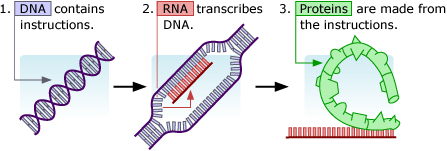
\includegraphics[scale=1]{figures/Agge/dnarnaprotein.png} 
\end{figure}
  
  \item Instead of the cells always splitting up after self replication, some stated to form more complex multi-celled organisms, the beginning of multi-cellular organisms.
\end{enumerate} \par

This was a short investigation into how life on earth could have evolved. Some of the hypotheses are still investigated and some gaps are still to be filled. An example of this is how RNA and proteins where created, because nucleic acids for DNA and RNA productions depend on proteins, but to build proteins nucleic acids are needed. The solution to this problem was first recently discovered, where the knowledge on RNA was expanded, and is was discovered that RNA is able to both store and copy itself concluding that nucleic acids came first \footnote{$http://evolution.berkeley.edu/evolibrary/article/side-0-0/origsoflife-01$24-05-2016}. \par

Many of these processes are dependent on energy from the sun, and it was after the first stromatolites and their photosynthesis the atmosphere started changing and became more oxygen rich. This will have worked as a toxic gas on some anaerobic cells, making aerobic cells more common on land. This just shows how many factors play a role on how life originated and further evolved, killing the first evidence of life as other life forms evolved.\par
From all of this a conclusion can be drawn in what might be expected to be found on Europa, a uplifting clue is found in the black smokers on Earth, which could be found on the bottom of Europa. But from what we see on earth, the most likely life forms are bacteria, or simple multi-cellular life forms, and what we need to look for includes, simple organic compounds, such as carbohydrates, enzymes, lipids fatty acids, nucleic acids, proteins, peptides, amino acids are some of the important compounds which could indicate life or a habitat for life.\par  
Another way to investigate life, is to look at the environment it is created from/in, and if life did exists we might see reminisce of life. The next two chapters look into the life harboring conditions and possible clues to look for from extinct life forms. \par

\subsection{Life harboring conditions and planetary habitability}
This chapter will look into the condition need for life to evolve on a planet, and since life beyond Earth is unknown, the theories on planetary habitability are built on what is known from Earth.\par
Planetary habitability, is a measure of a planet’s ability to harbour life in a habitable environment\footnote{$https://en.wikipedia.org/wiki/Planetary_habitability$ 24-05-2016}, this does not mean that life exists on the planet in question, but just that the conditions are right for life to develop, or to be transferred from another planet.\par 
Some of the requirement for life has already been discussed previously, but show up again in this chapter. One of them is energy, there need to be some sort of energy present, apart from that many other geophysical and astrophysical criteria must be just right, for a planet, to be habitable. Looking at one of NASA’s guide rules for life is “extend regions of liquid water\footnote{$http://www.nasa.gov/jpl/the-solar-system-and-beyond-is-awash-in-water$ 24-05-2016}”  since this is a great place for organic matter to form from, and here energy can come from either the sun in the top ocean layers, or for example black smokers on the bottom.\par
Habitability is not only dependent on the planets environment, atmosphere and so on, but also other externals needs to be considered; here we need to look at the astrophysical properties such as orbit and placement compared to the sun. In all there are many aspects to take in to account and like the chapter about “Defining life” some properties for habitability of a planet can be made:\par

\begin{enumerate}
\item Mass

\item Orbit and rotation

\item Geochemistry

\item Microenvironments and extremophiles

\end{enumerate} \par

The mass of a planet is important to sustaining an atmosphere; this is not a problem on Europa since the life is not expected to be found in its thin atmosphere. With smaller planets the energy left over from creation is lost faster making the planet geologically dead, this is a problem, since life is so dependent on an energy source. In the case of Europa the mass is very little compared to Earth which might point to a geological dead planet, and the energy must therefore come from the ice or the gravitational pull of Jupiter. But this does not always hold true, look at Jupiter’s other moon Io, is geological active, and even with its little mass. This activity comes from the gravity pull from Jupiter. \par
In the orbit stability is key; a stable orbit gives stability to the environment on the planet. The speed of rotation and how elliptic the orbit is, influences the temperatures on the planet, here stable temperatures are favorable, so half the planet is not frozen half the year and boiled the next half year. Looking at Europa the problem is not that impotent, since if life is found, it is located in the water protected by the sounding ice. \par
The geochemistry tells if the fundamental building blocks are present to create the “food” for living organisms. The four important elements from know from Earth are nitrogen, hydrogen, carbon and oxygen. It was already discussed in the chapter about life origin why these are important.  It is hard to tell if these are present in the ocean on Europa, a NASA study describe the “Why look at Europa” describes how hydrogen and oxygen might be present in just the right quantities.\par

When looking at a new planet maybe only a small part of it is habitable, comparing with Earth 3.5 billion years ago, life was not as abundant as it is now. Therefore a small sample from Earth would not have shown any sign of life, even if there was in some extreme place such as at the black smokers on the ocean floor. On Earth organisms know as extremophiles live in these very niche environments with conditions not suitable for “normal” life, there can be temperatures above 100 degrees Celsius, or very acidic/alkaline conditions. This expands the possibility of finding life in more extreme environments such as on Europa. \par
All of this can be summarized in a list of factors; the list was originally made for reproducing and survival of Earth microbes on Mars. The list has been modified to match an environment with no atmosphere\footnote{$http://mepag.jpl.nasa.gov/reports/MEPAG-SR-SAG-final1.pdf$ page 17 24-05-2016}.

\begin{itemize}
   \item  Water availability and activity
   \begin{itemize}
     \item  Activity of liquid water
     \item Past/further liquid (ice)
     \item Salinity and pH
    \end{itemize}
   \end{itemize}
   
     \begin{itemize}
       \item  Chemical environment
       
       \begin{itemize}
         \item Nutrients 
         
         \begin{itemize}
          \item C, H, N, O, P, S, essential metals and micronutrients
          \item Fixed nitrogen
          \item Their availability/mineralogy
         \end{itemize}
          
         \item Toxin
          \begin{itemize}
           \item Heavy metals (Zn, Ni, Cu, Cr, As, Cd, ect.
           \item Globally distributed oxidizing soils
          \end{itemize}
          
       \end{itemize}
     \end{itemize}
     
     \begin{itemize}
       \item  Energy for metabolisms 
       
       \begin{itemize}
         \item Solar/Radiation 
         \item Geochemical
         
         \begin{itemize}
          \item Oxidants
          \item Reductants
          \item Redox processes
         \end{itemize}
          
       \end{itemize}
     \end{itemize}
     
     \begin{itemize}
       \item  Physical condition 
       
       \begin{itemize}
         \item Temperature 
         \item Small temperature fluctuations
         \item High CO2 concentrations
         \item Water/ice flow
           
       \end{itemize}
     \end{itemize}
   
This list gives a good yard stick for determining if the planet is habitable, when Earth life forms are considered. Of cause life could be of a whole other unknown type which today’s technology cannot detect and this will give problems which is left out of this discussion. \par

\subsection{Extinct life}
Due to the small size of Europa, it might be geologically dead, but life might have thrived when the planet still had left over energy from its creation. Therefore it would be an idea to look for signs of extinct life, as we also see from Earth, previous life literally fuels today’s world. \par
When look for extinct life the search for distinct bio-makers/features that would indicate that life once thrived here. The things too look for will be leftovers from living organisms, this includes reduced carbon and nitrogen (CO3(2-), NO3-, NO2-, SO4(-2), also some important metals would be of interest Mg, Mn and Fe. But some of these compounds might not come from extinct life and it is therefore important to distinguish between biologically and not biologically produced compounds. An example of this is seen in the way N2 is deposited, with no biological processes the N2 would become NO2- and NO3-, but if this is used on a biological process it would form N2O or N2 as a gas  (dependent on pressure)\footnote{http://www.ncbi.nlm.nih.gov/pubmed/11537366 25-05-2016}. \par
From earth we see the extinct life in great quantizes such as olie and natural gas, produced by decomposing plants and animal matter under high heat and pressure. Natural gas is mainly made up of methane which would be a good marker for primordial life. Also olies floating on the water would indicate extinct life. \par

Through the last few chapters discussions about what life is and some of the signs to look out for have been investigated. Some of the findings have been applied to Europa and how it might fit the criteria as a life harbouring moon. In the last chapter a discussion about why Europa could be the place to go, for finding alien life in our solar system.\par

\subsection{Why look at Europa}

One of the most important properties of Europa is the liquid water found under the ice, which is key to life according to NASA, the more questionable, but just as important, is the energy need to create and sustain life. As discussed due to the small mass of Europa it might not be geologically active, if this is the case then a new NASA study carried out by JPL\footnote{$http://www.jpl.nasa.gov/news/news.php?feature=6514$ 25-05-2016} show that even without volcanic activity such as hydrothermal vents/black smokers, the balance of chemical energy might be there to support life. The study is based on methods know from Earth, and look at how energy and nutrients are carried around Earth’s oceans. But most importantly how the production of hydrogen and oxygen will take place without volcanic activity, one of the methods fro creating oxygen is serpentinization, where water reacts with freshly exposed rock (cracks form when cooling or water movement) to produce hydrogen. \par
The other part of the study looks in to the production of oxidants and oxygen, here the radiation from Jupiter splits ice/water on the surface, which cycles into the ice and down to the ocean. Scientist does believe that compounds from the top ice slowly cycles through the icy surface. If the amount of oxidants and hydrogen produced Europa is balnced just right, it might have just the right conditions to sustain life. \par
It is already know that Io has volcanic activity due to the Jupiter’s gravity push and pull on the rocky moon. This could indicate volcanic activity on Europa, giving even better conditions for life, due to the energy volcanic activity would bring. If Europa is geologically active there is a good chance of finding black smokers on the seafloor, this is one very important niche environment where life would thrive on the energy source and nutrients the black smokers produce.\par
Europa therefore seems like a perfect place to look for life and is also classified as a class III habitat. A planet in class III has liquid water of some sort trapped in or by ice, but since the water is enclosed the nutrient might be found in too small concentration to contain living organisms. This is the main problem with class III planet/moon, the lack of ingredients for life in one location due to the large water body and therefore lack of an incubator for life with the right amount of nutrients. \par
A illustration of all the possible methods for life to form is showed in the picture below, here radiation, ice cycle and volcanic activity would lead to a possible habitat for life in the ocean of Europa:\par

\begin{figure}[H]
\caption{The different process that Europa might have for producing a habitat for life}
\centering
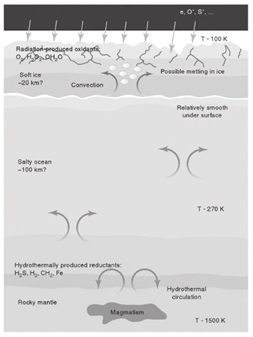
\includegraphics[scale=1]{figures/Agge/Europasurface.png} 
\end{figure}

In conclusion life is very complex to quantify and only a set of guidelines can be set up, derived from the life known to Earth. The guidelines set up give an indication of what to look for, when searching for a habitat or life on another planet, it also points to more precise investigations into what life forms might be found on Europa. It is still difficult to say anything exact of what could be expected to be found on Europa, in form of geology and energy source, but throughout this study it is evident that Europa is a good place the search for life in our solar system. In all Europa ticks many of the right boxes set up for a habitable moon with nutrition and energy to sustain life.


%* Water, oil, fat, carbon, energy
%
%* Proteins (amino acids) etc
%
%* Nutritions, water, heat energy
%
%* How can a life-form be able to convert thermal energy to other forms of energy
%
%* Another energy source could be geysers on the solid core
%
%    * A probe to the ocean bottom might show this
%    
%* Lakes inside the ice
%
%* Iron-reduction
